%!TEX root = bachelor.tex

\chapter{Evaluation}
\label{evaluation}

\subsubsection{Expectations and Methodology}

The efficiency of the different distribution models is already discussed theoretically in Chapter \ref{theory}. While the trade-offs are already known, the implementation of these models can cause unexpected side effects, which could have an impact on performance. The main goal of this evaluation is to verify, that the implementation of the Chunked-Swarm model is able to keep the $2\:T_0$ limit in practice, as predicted in Section \ref{theory:model:chunkedswarm}.

Therefore, the Benchmark module is used to simulate certain scenarios and thus to measure the influence of certain parameters like number of peers, upload and download bandwidth, chunk count and so on. The Monitoring module, see Section \ref{module:monitoring}, is used to record the current upload and download bandwidth and completion time of each peer during the benchmarks.

In order to get meaningful results, every scenario using the Chunked-Swarm model runs ten times, except those, which use the Sequential and Logarithmic model, because these models behave always predictable. In case of scenarios using the Chunked-Swarm model, the results are merged by calculating the mean and the confidence interval using a condidence level of 95\,\% of all runs. All results are plotted using gnuplot.

There are twelve scenarios in total. The first scenario is considered the default, while the remaining scenarios are variations of it. To measure the influence of each parameter, the scenarios have always only one parameter, that is different to the default scenario. All scenarios run on a virtual server with 14 \emph{Intel Xeon} 2.1 Ghz cores and 38 GB main memory.

\begin{figure}[!ht]
	\begin{center}	
		\subfigure[Completion\label{fig:s1:completion}]{
	 		\includegraphics[width=0.5\textwidth]{plots/scenario_1_default/plots/GeneratedMeanChunkCompletion.csv}
	 	}~ % No whitespace here!
	 	\subfigure[Completion Per Peer\label{fig:s1:scompletion}]{
	 		\includegraphics[width=0.5\textwidth]{plots/scenario_1_default/plots/GeneratedMeanSortedChunkCompletion.csv}
	 	}		

	 	\subfigure[Super Seeder Upload Bandwidth\label{fig:s1:ssupload}]{
	 		\includegraphics[width=0.5\textwidth]{plots/scenario_1_default/plots/GeneratedMeanCurrentSuperSeederUploadBandwidth.csv}
	 	}~ % No whitespace here!
	 	\subfigure[Seeder Upload Bandwidth\label{fig:s1:upload}]{
	 		\includegraphics[width=0.5\textwidth]{plots/scenario_1_default/plots/GeneratedMeanCurrentUploadBandwidth.csv}
	 	}

	 	\subfigure[Leecher Download Bandwidth\label{fig:s1:download}]{
	 		\includegraphics[width=0.5\textwidth]{plots/scenario_1_default/plots/GeneratedMeanCurrentDownloadBandwidth.csv}
	 	}
		\caption{Scenario 1 - Default}
		\label{fig:s1}
	\end{center}
\end{figure}


\subsubsection{Scenario 1: Default}


Scenario 1 simulates 64 peers using the Chunked-Swarm model, as explained in Section \ref{theory:model:chunkedswarm}, with super seeder extension, see Section \ref{module:algorithm:chunkedswarm}, where one peer has the complete data set at the beginning, which is called the super seeder and does only upload each chunk once. Every peer has a simulated upload bandwidth of $16.384\:\frac{bytes}{seconds}$. The download bandwidth is not limited. The size of the data set is not specified directly, but is calculated from the upload bandwidth and $T_0$, which is set to ten minutes (600 seconds). So a single transfer from the super seeder to one peer takes exactly $T_0$ seconds. The small upload bandwidth has a major advantage for benchmarking, because basically it represents the buffer size of each peer. So $n\:*\:u$ is the minimal memory usage of a benchmark, where $n$ is the number of peers and $u$ the upload bandwidth. If the upload bandwidth is too high, the overhead of the memory usage will influence the expressiveness of the benchmark. Since the size of the data set is always relative to the upload bandwidth and $T_0$, the actual upload bandwidth does not matter. The data set is also splitted into twice as many chunks as there are peers, but without the super seeder, which makes $63\:*\:2=126$ chunks. This scenario also simulates a meta data size of one byte. In reality, the meta data would be something about 64 bytes, because it contains a \emph{SHA-1} hash, a bit set and some network protocol headers, but because the upload bandwidth is reduced for the benchmark, the meta data size should be reduced as well. In this special case the $\frac{16.384\:\frac{bytes}{seconds}}{1\:byte}$ ratio is equal to $\frac{1.048.576\:\frac{bytes}{seconds}}{64\:bytes}$. So if we assume, that a usual peer has an upload bandwidth of $1.048.576\:\frac{bytes}{second}$, which is quite common these days, the benchmark values are realistic.

Figure \ref{fig:s1:completion} shows the mean completion graph for each peer, where the x-axis represents the time and the y-axis the completion of the data set from $0.0$ to $1.0$. After $1.5\:*\:T_0$ every peer has the complete data set available. As shown in Chapter \ref{theory}, the formula $T(n, c) = (1\:+\:\frac{n-1}{c})\:T_0$ calculates the time needed for the Chunked-Swarm model. So $c\:=126$, $n\:=\:63$ and $T(63, 126) = (1\:+\:\frac{63-1}{126})\:T_0 = 1,49\:T_0$. Figure \ref{fig:s1:scompletion} shows the mean completion time of all 63 peers, sorted in descending order. Since this graph is almost a horizontal line, all peers complete the transfer roughly at the same time.

Figure \ref{fig:s1:ssupload} shows the mean super seeder upload bandwidth. For $T_0$ seconds, the super seeder uploads at full speed after which it stops uploading, because the super seeder extension forbids uploading the same chunk twice, so every chunk is uploaded once. Figure \ref{fig:s1:upload} and Figure \ref{fig:s1:download} present the mean upload and download bandwidth of all remaining peers. Since there are twice as many chunks as peers, each peer can start uploading chunks after $0.5\:*\:T_0$ seconds, as described in Section \ref{theory:model:chunkedswarm}. It is important to note, that the super seeder and the remaining peers upload in parallel after $0.5\:*\:T_0$ seconds.



\begin{figure}[ht]
	\begin{center}
		\subfigure[Completion\label{fig:s2:completion}]{
	 		\includegraphics[width=0.5\textwidth]{plots/scenario_2_seq/plots/GeneratedMeanChunkCompletion.csv}
	 	}~ % No whitespace here!
	 	\subfigure[Completion\label{fig:s2:scompletion}]{
	 		\includegraphics[width=0.5\textwidth]{plots/scenario_2_seq/plots/GeneratedMeanSortedChunkCompletion.csv}
	 	}	 	

		\subfigure[Leecher Download Bandwidth\label{fig:s2:download}]{
	 		\includegraphics[width=0.5\textwidth]{plots/scenario_2_seq/plots/GeneratedMeanCurrentDownloadBandwidth.csv}
	 	}~ % No whitespace here!
	 	\subfigure[Super Seeder Upload Bandwidth\label{fig:s2:ssupload}]{
	 		\includegraphics[width=0.5\textwidth]{plots/scenario_2_seq/plots/GeneratedMeanCurrentSuperSeederUploadBandwidth.csv}
	 	}

		\caption{Scenario 2 - Sequential}
		\label{fig:s2}
	\end{center}
\end{figure}

\pagebreak
\subsubsection{Scenario 2: Sequential}

Scenario 2 uses the Sequential model, as explained in Section \ref{theory:model:sequential}, so there is only one seeder, which is uploading. This seeder is also called super seeder, though it is not related to the super seeder extension of the Chunked-Swarm model. This super seeder uploads data sets sequentially to all connected peers, which do not distribute these data sets among themselves. This scenario represents a client\,/\,server system, where the upload bandwidth is shared by all connected peers. All other parameters are taken from Scenario 1. As exptected, all peers need approximately $63\:*\:T_0$ seconds to complete the transfer, as shown in figure \ref{fig:s2:completion} and \ref{fig:s2:scompletion}. This makes sense, because every peer can only download with $\frac{16.384}{63}=267\:\frac{bytes}{second}$, while the super seeder uploads at full speed, see figure \ref{fig:s2:download} and \ref{fig:s2:ssupload}. The peaks in the upload and download bandwidth graphs are caused by the leaky-bucket algorithm used by the traffic shaping mechanism, see \ref{module:core:net:traffic}, and have no impact on performance.




\begin{figure}[!ht]
	\begin{center}	
		\subfigure[Completion\label{fig:s3:completion}]{
	 		\includegraphics[width=0.5\textwidth]{plots/scenario_3_log/plots/GeneratedMeanChunkCompletion.csv}
	 	}~ % No whitespace here!
	 	\subfigure[Completion Per Peer\label{fig:s3:scompletion}]{
	 		\includegraphics[width=0.5\textwidth]{plots/scenario_3_log/plots/GeneratedMeanSortedChunkCompletion.csv}
	 	}		

	 	\subfigure[Super Seeder Upload Bandwidth\label{fig:s3:ssupload}]{
	 		\includegraphics[width=0.5\textwidth]{plots/scenario_3_log/plots/GeneratedMeanCurrentSuperSeederUploadBandwidth.csv}
	 	}~ % No whitespace here!
	 	\subfigure[Seeder Upload Bandwidth\label{fig:s3:upload}]{
	 		\includegraphics[width=0.5\textwidth]{plots/scenario_3_log/plots/GeneratedMeanCurrentUploadBandwidth.csv}
	 	}

	 	\subfigure[Leecher Download Bandwidth\label{fig:s3:download}]{
	 		\includegraphics[width=0.5\textwidth]{plots/scenario_3_log/plots/GeneratedMeanCurrentDownloadBandwidth.csv}
	 	}
		\caption{Scenario 3 - Logarithmic}
		\label{fig:s3}
	\end{center}
\end{figure}

\pagebreak
\subsubsection{Scenario 3: Logarithmic}

Scenario 3 uses the Logarithmic model. As explained in Section \ref{theory:model:logarithmic}, this model uses a peer-to-peer network, like the Chunked-Swarm model, but only complete data sets are tranferred and a single peer only uploads to one other peer in parallel. Only one peer has the complete data set at first, which is also called the super seeder. This way, the number of uploading peers doubles every $T_0$ seconds, so the number of uploading and completed peers grows exponentially, see figure \ref{fig:s3:completion} and \ref{fig:s3:scompletion}. But it also means, that there are never more than 50\,\% of all peers uploading in parallel, which is shown in figure \ref{fig:s3:upload} and \ref{fig:s3:download}. Figure \ref{fig:s3:ssupload} presents the super seeder upload bandwidth including some rough peaks, which are caused by the announce delay. When a peer completes a download, it takes a few seconds to notify the remaining peers in the network. During this time the super seeder is not uploading anything, so these peaks are actually expected. Like Scenario 2, the minor peaks are part of the traffic shaping mechansim.

\vfill


\pagebreak
\begin{figure}[!ht]
	\begin{center}	
		\subfigure[Completion\label{fig:s4:completion}]{
	 		\includegraphics[width=0.5\textwidth]{plots/scenario_8_peer_count_32/plots/GeneratedMeanChunkCompletion.csv}
	 	}~ % No whitespace here!
	 	\subfigure[Completion Per Peer\label{fig:s4:scompletion}]{
	 		\includegraphics[width=0.5\textwidth]{plots/scenario_8_peer_count_32/plots/GeneratedMeanSortedChunkCompletion.csv}
	 	}		

	 	\subfigure[Super Seeder Upload Bandwidth\label{fig:s4:ssupload}]{
	 		\includegraphics[width=0.5\textwidth]{plots/scenario_8_peer_count_32/plots/GeneratedMeanCurrentSuperSeederUploadBandwidth.csv}
	 	}~ % No whitespace here!
	 	\subfigure[Seeder Upload Bandwidth\label{fig:s4:upload}]{
	 		\includegraphics[width=0.5\textwidth]{plots/scenario_8_peer_count_32/plots/GeneratedMeanCurrentUploadBandwidth.csv}
	 	}

	 	\subfigure[Leecher Download Bandwidth\label{fig:s4:download}]{
	 		\includegraphics[width=0.5\textwidth]{plots/scenario_8_peer_count_32/plots/GeneratedMeanCurrentDownloadBandwidth.csv}
	 	}
		\caption{Scenario 4 - 32 Peers}
		\label{fig:s4}
	\end{center}
\end{figure}
\vfill

\pagebreak
\begin{figure}[!ht]
	\begin{center}	
		\subfigure[Completion\label{fig:s5:completion}]{
	 		\includegraphics[width=0.5\textwidth]{plots/scenario_4_peer_count_128/plots/GeneratedMeanChunkCompletion.csv}
	 	}~ % No whitespace here!
	 	\subfigure[Completion Per Peer\label{fig:s5:scompletion}]{
	 		\includegraphics[width=0.5\textwidth]{plots/scenario_4_peer_count_128/plots/GeneratedMeanSortedChunkCompletion.csv}
	 	}		

	 	\subfigure[Super Seeder Upload Bandwidth\label{fig:s5:ssupload}]{
	 		\includegraphics[width=0.5\textwidth]{plots/scenario_4_peer_count_128/plots/GeneratedMeanCurrentSuperSeederUploadBandwidth.csv}
	 	}~ % No whitespace here!
	 	\subfigure[Seeder Upload Bandwidth\label{fig:s5:upload}]{
	 		\includegraphics[width=0.5\textwidth]{plots/scenario_4_peer_count_128/plots/GeneratedMeanCurrentUploadBandwidth.csv}
	 	}

	 	\subfigure[Leecher Download Bandwidth\label{fig:s5:download}]{
	 		\includegraphics[width=0.5\textwidth]{plots/scenario_4_peer_count_128/plots/GeneratedMeanCurrentDownloadBandwidth.csv}
	 	}
		\caption{Scenario 5 - 128 Peers}
		\label{fig:s5}
	\end{center}
\end{figure}
\vfill

\pagebreak
\begin{figure}[!ht]
	\begin{center}	
		\subfigure[Completion\label{fig:s6:completion}]{
	 		\includegraphics[width=0.5\textwidth]{plots/scenario_11_peer_count_192_v2/plots/GeneratedMeanChunkCompletion.csv}
	 	}~ % No whitespace here!
	 	\subfigure[Completion Per Peer\label{fig:s6:scompletion}]{
	 		\includegraphics[width=0.5\textwidth]{plots/scenario_11_peer_count_192_v2/plots/GeneratedMeanSortedChunkCompletion.csv}
	 	}		

	 	\subfigure[Super Seeder Upload Bandwidth\label{fig:s6:ssupload}]{
	 		\includegraphics[width=0.5\textwidth]{plots/scenario_11_peer_count_192_v2/plots/GeneratedMeanCurrentSuperSeederUploadBandwidth.csv}
	 	}~ % No whitespace here!
	 	\subfigure[Seeder Upload Bandwidth\label{fig:s6:upload}]{
	 		\includegraphics[width=0.5\textwidth]{plots/scenario_11_peer_count_192_v2/plots/GeneratedMeanCurrentUploadBandwidth.csv}
	 	}

	 	\subfigure[Leecher Download Bandwidth\label{fig:s6:download}]{
	 		\includegraphics[width=0.5\textwidth]{plots/scenario_11_peer_count_192_v2/plots/GeneratedMeanCurrentDownloadBandwidth.csv}
	 	}
		\caption{Scenario 6 - 192 Peers}
		\label{fig:s6}
	\end{center}
\end{figure}
\vfill

\pagebreak
\subsubsection{Scenario 4, 5 and 6: Peer Count}

Compared to the default scenario, scenario 4, 5 and 6 have a peer count of 32, 128 and 192 respectively. These scenarios are used to observe the large-scale behavior, whose results are shown in figure \ref{fig:s4}, \ref{fig:s5} and \ref{fig:s6}. The results from scenario 4 and the default scenario are almost identical, actually scenario 4 behaves even more as predicted. In contrast, scenario 5 and 6 show a minor decrease in performance. While the default scenario and scenario 4 both take about $1.5\:*\:T_0$ seconds, scenario 5 and 6 take $1.6\:*\:T_0$ and $1.7\:*\:T_0$ seconds respectively. While all of these scenarios do not exceed $2\:*\:T_0$ seconds, the performance obviously drops when using more peers.

The complexity of a mesh topology is ${\mathcal O(n^2)}$, which is one reason for the performance drop. If the peer count is doubled, the chunk count is doubled as well, so the number of announce messages actually quadruples. Theoretically, the Chunked-Swarm model works for any number of clients, but in practice the overhead introduced by the growing number of chunks and announce messages is just too high at some point. In reality, every announce message would also increase the latency caused by the \emph{round trip time}. 

Another reason might be unfair chunk distribution, because if a peer downloads its chunk too fast, it might download a second chunk, which should have been distributed by an other peer and thus distributes two chunks instead of one. This effect seems to happen more often under high pressure, as shown in figure \ref{fig:s5:upload} and \ref{fig:s6:upload}. Some peers start distributing their own chunks before $0.5\:*\:T_0$, while others seem to upload chunks even after $1.5\:*\:T_0$. A solution to this problem is discussed in Chapter \ref{conclusion}.

It should be noted, that the limit is not exactly 192 peers. When simulating 192 peers, the server actually runs $192\:*\:191=36.672$ connections at once, which has a great impact on CPU and main memory usage. Programmatically, there are also major reasons for the huge overhead. Since the implementation is written in Java, there is no way to allocate class instances on the stack. This is discussed in Chapter \ref{conclusion} in more detail. Also, in reality, the overhead is distributed evenly among all peers. So a single peer should be able to handle way more than 192 peers. Unfortunately, there are no results taken from real peers yet, so the last statement is just an assumption, which has yet to be proven.

\vfill



\pagebreak
\begin{figure}[!ht]
	\begin{center}	
		\subfigure[Completion\label{fig:s7:completion}]{
	 		\includegraphics[width=0.5\textwidth]{plots/scenario_7_chunk_count_fac_1/plots/GeneratedMeanChunkCompletion.csv}
	 	}~ % No whitespace here!
	 	\subfigure[Completion Per Peer\label{fig:s7:scompletion}]{
	 		\includegraphics[width=0.5\textwidth]{plots/scenario_7_chunk_count_fac_1/plots/GeneratedMeanSortedChunkCompletion.csv}
	 	}		

	 	\subfigure[Super Seeder Upload Bandwidth\label{fig:s7:ssupload}]{
	 		\includegraphics[width=0.5\textwidth]{plots/scenario_7_chunk_count_fac_1/plots/GeneratedMeanCurrentSuperSeederUploadBandwidth.csv}
	 	}~ % No whitespace here!
	 	\subfigure[Seeder Upload Bandwidth\label{fig:s7:upload}]{
	 		\includegraphics[width=0.5\textwidth]{plots/scenario_7_chunk_count_fac_1/plots/GeneratedMeanCurrentUploadBandwidth.csv}
	 	}

	 	\subfigure[Leecher Download Bandwidth\label{fig:s7:download}]{
	 		\includegraphics[width=0.5\textwidth]{plots/scenario_7_chunk_count_fac_1/plots/GeneratedMeanCurrentDownloadBandwidth.csv}
	 	}
		\caption{Scenario 7 - Chunk Count Factor 1}
		\label{fig:s7}
	\end{center}
\end{figure}
\vfill

\pagebreak
\begin{figure}[!ht]
	\begin{center}	
		\subfigure[Completion\label{fig:s8:completion}]{
	 		\includegraphics[width=0.5\textwidth]{plots/scenario_15_chunk_count_fac_4/plots/GeneratedMeanChunkCompletion.csv}
	 	}~ % No whitespace here!
	 	\subfigure[Completion Per Peer\label{fig:s8:scompletion}]{
	 		\includegraphics[width=0.5\textwidth]{plots/scenario_15_chunk_count_fac_4/plots/GeneratedMeanSortedChunkCompletion.csv}
	 	}		

	 	\subfigure[Super Seeder Upload Bandwidth\label{fig:s8:ssupload}]{
	 		\includegraphics[width=0.5\textwidth]{plots/scenario_15_chunk_count_fac_4/plots/GeneratedMeanCurrentSuperSeederUploadBandwidth.csv}
	 	}~ % No whitespace here!
	 	\subfigure[Seeder Upload Bandwidth\label{fig:s8:upload}]{
	 		\includegraphics[width=0.5\textwidth]{plots/scenario_15_chunk_count_fac_4/plots/GeneratedMeanCurrentUploadBandwidth.csv}
	 	}

	 	\subfigure[Leecher Download Bandwidth\label{fig:s8:download}]{
	 		\includegraphics[width=0.5\textwidth]{plots/scenario_15_chunk_count_fac_4/plots/GeneratedMeanCurrentDownloadBandwidth.csv}
	 	}
		\caption{Scenario 8 - Chunk Count Factor 4}
		\label{fig:s8}
	\end{center}
\end{figure}
\vfill

\pagebreak
\begin{figure}[!ht]
	\begin{center}	
		\subfigure[Completion\label{fig:s9:completion}]{
	 		\includegraphics[width=0.5\textwidth]{plots/scenario_16_chunk_count_fac_8/plots/GeneratedMeanChunkCompletion.csv}
	 	}~ % No whitespace here!
	 	\subfigure[Completion Per Peer\label{fig:s9:scompletion}]{
	 		\includegraphics[width=0.5\textwidth]{plots/scenario_16_chunk_count_fac_8/plots/GeneratedMeanSortedChunkCompletion.csv}
	 	}		

	 	\subfigure[Super Seeder Upload Bandwidth\label{fig:s9:ssupload}]{
	 		\includegraphics[width=0.5\textwidth]{plots/scenario_16_chunk_count_fac_8/plots/GeneratedMeanCurrentSuperSeederUploadBandwidth.csv}
	 	}~ % No whitespace here!
	 	\subfigure[Seeder Upload Bandwidth\label{fig:s9:upload}]{
	 		\includegraphics[width=0.5\textwidth]{plots/scenario_16_chunk_count_fac_8/plots/GeneratedMeanCurrentUploadBandwidth.csv}
	 	}

	 	\subfigure[Leecher Download Bandwidth\label{fig:s9:download}]{
	 		\includegraphics[width=0.5\textwidth]{plots/scenario_16_chunk_count_fac_8/plots/GeneratedMeanCurrentDownloadBandwidth.csv}
	 	}
		\caption{Scenario 9 - Chunk Count Factor 8}
		\label{fig:s9}
	\end{center}
\end{figure}
\vfill


\pagebreak
\begin{figure}[!ht]
	\begin{center}	
		\subfigure[Completion\label{fig:s10:completion}]{
	 		\includegraphics[width=0.5\textwidth]{plots/scenario_17_chunk_count_fac_16/plots/GeneratedMeanChunkCompletion.csv}
	 	}~ % No whitespace here!
	 	\subfigure[Completion Per Peer\label{fig:s10:scompletion}]{
	 		\includegraphics[width=0.5\textwidth]{plots/scenario_17_chunk_count_fac_16/plots/GeneratedMeanSortedChunkCompletion.csv}
	 	}		

	 	\subfigure[Super Seeder Upload Bandwidth\label{fig:s10:ssupload}]{
	 		\includegraphics[width=0.5\textwidth]{plots/scenario_17_chunk_count_fac_16/plots/GeneratedMeanCurrentSuperSeederUploadBandwidth.csv}
	 	}~ % No whitespace here!
	 	\subfigure[Seeder Upload Bandwidth\label{fig:s10:upload}]{
	 		\includegraphics[width=0.5\textwidth]{plots/scenario_17_chunk_count_fac_16/plots/GeneratedMeanCurrentUploadBandwidth.csv}
	 	}

	 	\subfigure[Leecher Download Bandwidth\label{fig:s10:download}]{
	 		\includegraphics[width=0.5\textwidth]{plots/scenario_17_chunk_count_fac_16/plots/GeneratedMeanCurrentDownloadBandwidth.csv}
	 	}
		\caption{Scenario 10 - Chunk Count Factor 16}
		\label{fig:s10}
	\end{center}
\end{figure}
\vfill

\pagebreak
\subsubsection{Scenario 7, 8, 9 and 10: Chunk Count Factor}

In scenario 7, 8, 9 and 10 the chunk count factor is adjusted to 1, 4, 8 and 16 respectively. The chunk count factor is multiplied with the number of peers, but without the super seeder, to calculate the actual chunk count. The default scenario uses a chunk count factor of 2 and a peer count of 63, without the super seeder. Since these four scenarios only change the chunk count factor, the used chunk counts are $1\:*\:63$, $4\:*\:63=252$, $8\:*\:63=504$ and $16\:*\:63=1008$ for scenario 7, 8, 9 and 10 respectively.   

As expected, scenario 7 completes in $2\:*\:T_0$, see figure \ref{fig:s7}. In the first $T_0$ seconds the super seeder uploads a distinct chunk to each peer, whereby the complete data set is available in the network. Since the super seeder is not allowed to upload the same chunk twice, the peer have to distribute all chunks evenly among themselves, which also takes roughly $T_0$ seconds. These results correspond with the formula presented in \ref{theory:model:chunkedswarm}, because $c\:=63$, $n\:=\:63$ and $T(63, 63) = (1\:+\:\frac{63-1}{63})\:T_0 = 1,98\:T_0$.

Scenario 8, whose results are shown in figure \ref{fig:s8}, completed in $1.3\:*\:T_0$, which is almost the expected duration, since $c\:=252$, $n\:=\:63$ and $T(63, 252) = (1\:+\:\frac{63-1}{252})\:T_0 = 1,25\:T_0$. But it is important to note, that at with chunk count factor of 4, the completion graph already starts to leave the expected path, which should have been a step function with four steps, starting at $0.25\:*\:T_0$. As with Scenario 5 and 6, this effect gets worse under high pressure. The unfair chunk distribution also gets worse, if more chunks are involved. So while the overall distribution time shrinks, the system as a whole gets more fragile.

Scenario 9 and 10 are even more fragile, as shown in figure \ref{fig:s9} and \ref{fig:s10}. The expected durations are $(1\:+\:\frac{63-1}{504})\:T_0 = 1,12\:T_0$ and $(1\:+\:\frac{63-1}{1008})\:T_0 = 1,06\:T_0$ respectively. Even worse, scenario 10 takes longer than scenario 9 on average. While scenario 9 is barely acceptable, scenario 10 has a new influence, that should be noted. As explained before, the results are calculated from ten runs. At this point, all ten runs of all scenarios completed mostly identical, which is represented by the low confidence interval. This changes dramatically in scenario 10. Some runs completed at $1.5\:*\:T_0$, while the majority completed at $1.08\:*\:T_0$. This means, that some runs behaved much worse than the others. The raw results let assume, that unfair chunk distribution is now the main reason for that. Figure \ref{fig:s10:scompletion}, \ref{fig:s10:upload} and \ref{fig:s10:download} contain these high confidence interval areas. 

In theory, if the chunk count is doubled, the completion time after $T_0$ will cut in half. Scenario 1, 7, 8 and 9 confirm this assumption. But it seems, that unfair chunk distribution can make the system really fragile. Since this problem occurs under high pressure in every scenario, a more stable implementation has to be found.

\vfill


\pagebreak
\begin{figure}[!ht]
	\begin{center}	
		\subfigure[Completion\label{fig:s11:completion}]{
	 		\includegraphics[width=0.5\textwidth]{plots/scenario_9_parts_10/plots/GeneratedMeanChunkCompletion.csv}
	 	}~ % No whitespace here!
	 	\subfigure[Completion Per Peer\label{fig:s11:scompletion}]{
	 		\includegraphics[width=0.5\textwidth]{plots/scenario_9_parts_10/plots/GeneratedMeanSortedChunkCompletion.csv}
	 	}		

	 	\subfigure[Super Seeder Upload Bandwidth\label{fig:s11:ssupload}]{
	 		\includegraphics[width=0.5\textwidth]{plots/scenario_9_parts_10/plots/GeneratedMeanCurrentSuperSeederUploadBandwidth.csv}
	 	}~ % No whitespace here!
	 	\subfigure[Seeder Upload Bandwidth\label{fig:s11:upload}]{
	 		\includegraphics[width=0.5\textwidth]{plots/scenario_9_parts_10/plots/GeneratedMeanCurrentUploadBandwidth.csv}
	 	}

	 	\subfigure[Leecher Download Bandwidth\label{fig:s11:download}]{
	 		\includegraphics[width=0.5\textwidth]{plots/scenario_9_parts_10/plots/GeneratedMeanCurrentDownloadBandwidth.csv}
	 	}
		\caption{Scenario 11 - Streaming 10 Data Sets}
		\label{fig:s11}
	\end{center}
\end{figure}
\vfill


\pagebreak
\begin{figure}[!ht]
	\begin{center}	
		\subfigure[Completion\label{fig:s12:completion}]{
	 		\includegraphics[width=0.5\textwidth]{plots/scenario_6_parts_20/plots/GeneratedMeanChunkCompletion.csv}
	 	}~ % No whitespace here!
	 	\subfigure[Completion Per Peer\label{fig:s12:scompletion}]{
	 		\includegraphics[width=0.5\textwidth]{plots/scenario_6_parts_20/plots/GeneratedMeanSortedChunkCompletion.csv}
	 	}		

	 	\subfigure[Super Seeder Upload Bandwidth\label{fig:s12:ssupload}]{
	 		\includegraphics[width=0.5\textwidth]{plots/scenario_6_parts_20/plots/GeneratedMeanCurrentSuperSeederUploadBandwidth.csv}
	 	}~ % No whitespace here!
	 	\subfigure[Seeder Upload Bandwidth\label{fig:s12:upload}]{
	 		\includegraphics[width=0.5\textwidth]{plots/scenario_6_parts_20/plots/GeneratedMeanCurrentUploadBandwidth.csv}
	 	}

	 	\subfigure[Leecher Download Bandwidth\label{fig:s12:download}]{
	 		\includegraphics[width=0.5\textwidth]{plots/scenario_6_parts_20/plots/GeneratedMeanCurrentDownloadBandwidth.csv}
	 	}
		\caption{Scenario 12 - Streaming 20 Data Sets}
		\label{fig:s12}
	\end{center}
\end{figure}
\vfill

\pagebreak
\subsubsection{Scenario 11 and 12: Streaming Multiple Data Sets}

So far, all other scenarios used and transferred only one data set. The last scenarios 11 and 12 implement the streaming of 10 and 20 data sets respectively, see Section \ref{theory:model:chunkedswarm} and \ref{module:streaming}. The data sets are much smaller now and thus complete in less time.

In case of scenario 11, each data set takes $\frac{1}{10}\:*\:T_0$ seconds to get from one peer to another. So transferring all data sets take $T_0$ seconds. Therefore, the peers download ten data sets from the super seeder and distribute them one after the other. This is useful to implement sequential streaming, where a huge data source is splitted into multiple data sets, which are downloaded and distributed sequentially so that each peer do not have random chunks but a growing amount of coherent chunks instead. Video streaming is only one domain, which relies on this behavior.

Figure \ref{fig:s11} shows the results from scenario 11. An interesting observation is, that all peers finish within $1.2\:*\:T_0$ seconds, but each data set has a chunk count factor of 2. The reason is, that the download and the distribution phases of each data set interleave. So the super seeder starts uploading the next data set while the peers are still distributing the last data set, which is shown in figure \ref{fig:s11:ssupload}, \ref{fig:s11:upload} and \ref{fig:s11:download}. The high confidence intervals are caused by the large amount of chunks. When simulating ten runs, it is very unlikely, that all results are equal. But the confidence intervals show, that it is still very likely, that a further run will be very similar. The completion graphs \ref{fig:s11:completion} and \ref{fig:s11:scompletion} also show the good distribution behavior. All peers download and distribute the data sets equally. Figure \ref{fig:s12} contains the results from scenario 12, which has 20 data sets instead of 10. The results are very similar to those from scenario 11, so there is not much to say about it.

While the results of both scenarios look promising, it should be noted, that both scenarios run 20 times instead of 10. Then only the best 10 runs were chosen and merged. The reason is, that some runs took about $4\:*\:T_0$ to $6\:*\:T_0$ seconds to finish, while others took roughly $1.2\:*\:T_0$ seconds. In case of the slow scenarios, the results show, that most of the peers were not uploading anymore after $1.5\:*\:T_0$ seconds, which is the reason why these runs took so long. So the graphs of both scenarios show, that it is possible to get the expected performance, but the system is also very fragile and can get out of step. Again, the main reason for this effect is unfair chunk distribution. In the next Chapter \ref{conclusion} a push based approach is proposed, which should solve this particular problem in the future.
